\section{The $D_4$ example}
In this section we prove Theorem~\ref{D4example}. We use the triality of $D_4$ in an essential way.\\

Let $\tilde{G}$ be a simple algebraic group of type $D_4$ defined over a nonperfect field of characteristic $2$. Fix a maximal $k$-torus of $\tilde{G}$ and a $k$-defined Borel subgroup of $\tilde{G}$. let $\Psi(\tilde G)=\Psi(\tilde G,T)$ be the set of roots corresponding to $T$, and $\Psi(\tilde{G})^{+}=\Psi(\tilde{G},B,T)$ be the set of positive roots of $\tilde{G}$ corresponding to $T$ and $B$. The following Dynkin diagram defines the set of simple roots of $\tilde{G}$.
\begin{figure}[h]
                \centering
                \scalebox{0.7}{
                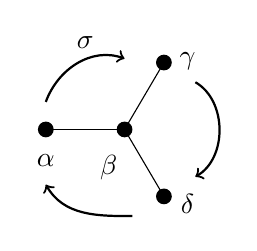
\begin{tikzpicture}
                \draw (1,0) to (2,0);
                \draw (2,0) to (2.5,0.85);
                \draw (2,0) to (2.5,-0.85);
                \fill (1,0) circle (1mm);
                \fill (2,0) circle (1mm);
                \fill (2.5,0.85) circle (1mm);
                \fill (2.5,-0.85) circle (1mm);
                \draw[below] (1,-0.2) node{$\alpha$};
                \draw[below] (1.8,-0.2) node{$\beta$};
                \draw[below] (2.8,1.1) node{$\gamma$};
                \draw[below] (2.8,-0.7) node{$\delta$};
                \draw [->,thick] (1.0,0.35) to [out=70,in=160] (2.0,0.9);
                \node (a) at (1.5, 1.1) {$\sigma$};
                \draw [->,thick] (2.9,0.6) to [out=-30,in=30] (2.9,-0.6);
                \draw [->,thick] (2.1,-1.1) to [out=180,in=-60] (1.0,-0.7);
               \end{tikzpicture}}
\end{figure}
Let $G:=\tilde{G}\rtimes \langle \sigma \rangle$ where $\sigma$ is the non-trivial element of the graph automorphism group of $\tilde{G}$ (normalizing $T$ and $B$) as the diagram defines; we have $\sigma\cdot \alpha=\gamma, \; \sigma\cdot \gamma=\delta, \; \sigma\cdot \delta=\alpha$, and $\beta$ is fixed by $\sigma$. We label $\Psi(\tilde{G})^{+}$ in the following. The corresponding negative roos are defined accordingly. Note that Roots 1, 2, 3, 4 correspond to $\alpha$, $\gamma$, $\delta$, $\beta$ respectively.

\begin{table}[!h]
\begin{center}
\scalebox{0.7}{
\begin{tabular}{cccccc}
\rootsD{1}{0}{1}{0}{0}&\rootsD{2}{1}{0}{0}{0}&\rootsD{3}{0}{0}{0}{1}&\rootsD{4}{0}{0}{1}{0}&\rootsD{5}{0}{1}{1}{0}&\rootsD{6}{1}{0}{1}{0}\\
\rootsD{7}{0}{0}{1}{1}&\rootsD{8}{1}{1}{1}{0}&\rootsD{9}{0}{1}{1}{1}&\rootsD{10}{1}{0}{1}{1}&\rootsD{11}{1}{1}{1}{1}&\rootsD{12}{1}{1}{2}{1}\\
\end{tabular}
}
\end{center}
\end{table}   

Define
$\lambda:=(\alpha+2\beta+\gamma+\delta)^{\vee}=\alpha^{\vee}+2\beta^{\vee}+\gamma^{\vee}+\delta^{\vee}$. 
Then 
\begin{alignat*}{2}
P_\lambda&=\langle T, \sigma, U_{\zeta}\mid \zeta\in \Psi(\tilde G)^{+}\cup \{-1,-2,-3\} \rangle,\\
L_\lambda&=\langle T, \sigma, U_{\zeta}\mid \zeta\in \{\pm 1,\pm 2,\pm 3\} \rangle,\\
R_u(P_\lambda)&=\langle U_{\zeta} \mid \zeta \in \Psi(\tilde G)^{+}\backslash \{1, 2, 3\} \rangle.
\end{alignat*}
Let $a\in k\backslash k^2$. Let $v(\sqrt a):=\epsilon_{6}(\sqrt a)\epsilon_{9}(\sqrt a)\in R_u(P_\lambda)(\overline k)$. Define
\begin{equation*}
H:=v(\sqrt a)\cdot\langle (n_{\alpha}\sigma), \; (\alpha+\gamma)^{\vee}(\overline k^*) \rangle.
\end{equation*}
Here is our first main result in this section.
\begin{prop}\label{firstmain}
$H$ is $k$-defined. Moreover, $H$ is $G$-cr but not $G$-cr over $k$. 
\end{prop}
\begin{proof}
First, we have 
$
(n_\alpha \sigma) \cdot (\beta+\delta) = (n_\alpha \sigma) \cdot 6 = 9, \;
(n_\alpha \sigma) \cdot 9 = 6.
$
Using this and the commutation relations~\cite[Lem.~32.5 and Prop.~33.3]{Humphreys-book1}, we obtain
\begin{equation*}
v(\sqrt a)\cdot (n_{\alpha}\sigma)=(n_\alpha \sigma) \epsilon_{12}(a).
\end{equation*}
An easy computation shows that $v(\sqrt a)$ commutes with $(\alpha+\gamma)^{\vee}(\overline k^*)$. Now it is clear that $H$ is $k$-defined. 

Now we show that $H$ is $G$-cr. It is sufficient to show that $H':=v(\sqrt a)^{-1}\cdot H=\langle n_\alpha \sigma,\; (\alpha+\gamma)^{\vee}(\overline k^*)$ is $G$-cr since it is $G$-conjugate to $H$. Since $H'$ is contained in $L_\lambda$, by Proposition~\ref{G-cr-L-cr} it is enough to show that $H'$ is $L_\lambda$-cr. We actually show that $H'$ is $L_\lambda$-ir. Note that $L_\lambda=A_1\times A_1 \times A_1=L_\alpha\times L_\gamma\times L_\delta$. We have 
\begin{equation*}
(n_\alpha \sigma)\cdot (\alpha+\gamma)^{\vee}(\overline k^*) = (\gamma+\delta)^{\vee}(\overline k^*),\;
(n_\alpha \sigma)^3 = n_\alpha n_\gamma n_\delta.
\end{equation*}  
Thus $H'$ contains $(\alpha+\gamma)^{\vee}(\overline k^*)$, $(\gamma+\delta)^{\vee}(\overline k^*)$, and $n_\alpha n_\gamma n_\delta$. Now it is clear that $H'$ is $L_\lambda$-ir. 

Next, we show that $H$ is not $G$-cr over $k$. Suppose the contrary. Clearly $H$ is contained in a $k$-defined $R$-parabolic subgroup $P_\lambda$. Then there exists a $k$-defined $R$-Levi subgroup of $P_\lambda$ containing $H$. Then by~\cite[Lem.~2.5(\rmnum{3})]{Bate-uniform-TransAMS} there exists $u\in R_u(P_\lambda)(k)$ such that $H$ is contained in $u\cdot L_\lambda$. Thus $n_\alpha\sigma\epsilon_{12}(a) < u\cdot L_\lambda$. So $u^{-1}\cdot (n_\alpha\sigma \epsilon_{12}(a)) < L_{\lambda}$. By~\cite[Prop.~8.2.1]{Springer-book}, we set
\begin{equation*}
u:=\prod_{\zeta\in \Psi(R_u(P_\lambda))}\epsilon_\zeta(x_\zeta).
\end{equation*}
We compute how $n_\alpha \sigma$ acts $\Psi(R_u(P_\lambda))$. Using the labelling of the positive roots above, we have $\Psi(R_u(P_\lambda))=\{4,\cdots 12\}$. We compute how $n_\alpha \sigma$ acts on $\Psi(R_u(P_\lambda))$: 
\begin{equation}\label{perm}
n_\alpha \sigma = (4\;5\;8\;11\;10\;7) (6\;9) (12). 
\end{equation}
Using this and the commutation relations,
\begin{alignat*}{2}
u^{-1}\cdot (n_\alpha\sigma \epsilon_{12}(a))
=&n_\alpha \sigma\epsilon_7(x_4+x_7)\epsilon_{10}(x_7+x_{10})\epsilon_{9}(x_6+x_9)\epsilon_{11}(x_{10}+x_{11})\\
&\epsilon_{6}(x_6+x_9)\epsilon_{8}(x_8+x_{11})\epsilon_{4}(x_4+x_5)\epsilon_{5}(x_5+x_8)\\
&\epsilon_{12}(x_5 x_{10}+x_{5}x_{11}+x_7 x_8 +x_7 x_{11}+x_8 x_{10}+{x_9}^2+a).
\end{alignat*}
Thus if $u^{-1}\cdot (n_\alpha\sigma \epsilon_{\alpha+2\beta+\gamma+\delta}(a)) < L_{\lambda}$ we must have
\begin{alignat*}{2}
&x_4=x_5=x_7=x_{8}=x_{10}=x_{11},\; x_6=x_9,\\
&x_5 x_{10}+x_{5}x_{11}+x_7 x_8 +x_7 x_{11}+x_8 x_{10}+{x_9}^2+a=0.
\end{alignat*}
Set $x_4=y$. Then we have $y^2+{x_9}^2+a=0$. Thus $(y+x_9)^2=a$. This is impossible since $y, x_9\in k$ and $a\notin k^2$. We are done. 
\end{proof}

\begin{rem}\label{D4nonsep}
From the computations above we see that the curve $C(x):=\{\epsilon_{6}(x)\epsilon_{9}(x)\mid x\in \overline k\}$ is not contained in $C_G(H)$, but the corresponding element in $\textup{Lie}(G)$, that is, $e_6+e_9$ is contained in $\mathfrak{c}_{\mathfrak{g}}(H)$. Then the argument in the proof of~\cite[Prop.~3.3]{Uchiyama-Separability-JAlgebra} shows that $\textup{Dim}(C_G(H))$ is strictly smaller than $\textup{Dim}(\mathfrak{c}_{\mathfrak{g}}(H))$. So $H$ is non-separable in $G$. 
\end{rem} 

\vspace{5mm}
Now we move on to the second main result in this section. We use the same $G$, $\lambda$, and $a$ as above. We also use the same labelling of the roots of $G$. Let $v(\sqrt a):=\epsilon_{-6}(\sqrt a)\epsilon_{-9}(\sqrt a)$. Let
\begin{equation*}
K:=v(\sqrt a)\cdot \langle n_{\alpha}\sigma,\; (\alpha+\gamma)^{\vee}(\overline k^*)\rangle=\langle n_\alpha \sigma \epsilon_{-12}(a), \;  (\alpha+\gamma)^{\vee}(\overline k^*)\rangle. 
\end{equation*}
Define
\begin{equation*}
H:=\langle K, \; \epsilon_{11}(1) \rangle.
\end{equation*}

\begin{prop}\label{secondmain}
$H$ is $k$-defined. Moreover, $H$ is $G$-ir over $k$ but not $G$-cr. 
\end{prop}
\begin{proof}
$H$ is clearly $k$-defined. First, we show that $H$ is $G$-ir over $k$. Note that
\begin{equation*}
v(\sqrt a)^{-1}\cdot H = \langle n_\alpha \sigma, \; (\alpha+\gamma)^{\vee}(\overline k^*),\; \epsilon_{11}(1)\epsilon_{2}(\sqrt a)\rangle.
\end{equation*}
Thus we see that $v(\sqrt a)^{-1}\cdot H$ is contained in $P_\lambda$. So $H$ is contained in $v(\sqrt a)\cdot P_\lambda$. 

\begin{lem}\label{uniquepara}
$v(\sqrt a)\cdot P_\lambda$ is the unique proper $R$-parabolic subgroup of $G$ containing $H$.
\end{lem}
\begin{proof}
Suppose that $P_\mu$ is a proper $R$-parabolic subgroup containing $v(\sqrt a)^{-1}\cdot H$. In the proof of Proposition~\ref{firstmain} we have shown that $M:=\langle n_\alpha \sigma, (\alpha+\gamma)^{\vee}(\overline k^*)\rangle$ is $G$-cr. Then there exists a $R$-Levi subgroup $L$ of $P_\mu$ containing $M$ since $M$ is contained in $P_\mu$. Since $R$-Levi subgroups of $P_\mu$ are $R_u(P_\mu)$-conjugate by~\cite[Lem.~2.5(\rmnum{3})]{Bate-uniform-TransAMS}, without loss, we set $L:=L_\mu$. Then $M<L_\mu=C_G(\mu(\overline k^*))$, so $\mu(\overline k^*)$ centralizes $M$. Recall that by~\cite[Thm.~13.4.2]{Springer-book}, $C_{R_u(P_\lambda)}(M)^{\circ}\times C_{L_\lambda}(M)^{\circ}\times C_{R_u(P_\lambda^{-})}(M)^{\circ}$ is an open set of $C_G(M)^{\circ}$ where $P_\lambda^{-}$ is the opposite of $P_\lambda$ containing $L_\lambda$.  
\begin{lem}\label{centralizerofM}
$C_G(M)^{\circ}=G_{12}$.
\end{lem}
\begin{proof}
First of all, from Equation~(\ref{perm}) we see that $G_{12}$ is contained in $C_G(n_\alpha \sigma)$. Since $\langle \alpha+2\beta+\gamma+\delta, (\alpha+\gamma)^{\vee} \rangle=0$, $G_{21}$ is also contained in $C_G((\alpha+\gamma)^{\vee}(\overline k^*))$. So $G_{12}$ is contained in $C_G(M)$. Set $u:=\prod_{i\in \Psi(R_u(P_\lambda))}\epsilon_{i}(x_i)$ for some $x_i \in \overline k$. Using Equation~\ref{perm} and the commutation relations, we obtain
\begin{alignat*}{2}
(n_\alpha \sigma)\cdot u &= \epsilon_{4}(x_7)\epsilon_{5}(x_4)\epsilon_{6}(x_9)\epsilon_7(x_{10})\epsilon_8(x_{5})\epsilon_9(x_6)\epsilon_{10}(x_{11})\epsilon_{11}(x_8)\epsilon_{12}(x_5 x_{10}+x_6 x_9 +x_{12}). 
\end{alignat*}
So, if $u\in C_{R_u(P_\lambda)}(n_\alpha \sigma)$ we must have
$x_4=x_5=x_7=x_{8}=x_{10}=x_{11},\; x_6=x_9$. But $\langle (\alpha+\gamma)^{\vee}, \alpha+\beta \rangle =2$, so $x_5=0$ for $u\in C_{R_u(P_\lambda)}(M)$. Then 
\begin{equation*}
(n_\alpha \sigma)\cdot u = \epsilon_6(x_6)\epsilon_9(x_6)\epsilon_{12}(x_6^2+x_{12}).
\end{equation*}
So we must have $x_6^2=0$ if $u\in C_{R_u(P_\lambda)}(M)$. Thus we conclude that $C_{R_u(P_\lambda)}(M)=U_{12}$. Similarly, we can show that $C_{R_u(P_{\lambda}^{-})}(M)=U_{-12}$. Now we show that $C_L(M)<G_{12}$. In the proof of Proposition~\ref{firstmain} we have shown that $(\gamma+\delta)^{\vee}(\overline k^*)$ is contained in $M$. So $C_{L_\lambda}(M)$ is contained in $C_{L_\lambda}((\alpha+\gamma)^{\vee}(\overline k^*),\; (\gamma+\delta)^{\vee}(\overline k^*))$. A direct computation shows that $C_{L_\lambda}((\alpha+\gamma)^{\vee}(\overline k^*),\; (\gamma+\delta)^{\vee}(\overline k^*)) = T$ and $C_T(n_\alpha \sigma)=(\alpha+2\beta+\gamma+\delta)^{\vee}(\overline k^*)<G_{12}$. We are done.
\end{proof}
Since $\lambda(\overline k^*)$ centralizes $M$, Lemma~\ref{centralizerofM} yields $\mu(\overline k^*)<G_{12}$. Then we can set $\mu:=g\cdot (\alpha+2\beta+\gamma+\delta)^{\vee}$ for some $g\in G_{12}$. By the Bruhat decomposition, $g$ is one of the following forms:
\begin{alignat*}{2}
&(1)\;g=(\alpha+2\beta+\gamma+\delta)^{\vee}(s)\epsilon_{12}(x_1),\\
&(2)\;g=\epsilon_{12}(x_1)n_{\alpha+2\beta+\gamma+\delta}(\alpha+2\beta+\gamma+\delta)^{\vee}(s)\epsilon_{12}(x_2)\\
&\textup{for some } x_1, x_2\in \overline k, s\in \overline k^*.
\end{alignat*}
We rule out the second case. Suppose $g$ is of the second form. Note that $\epsilon_{11}(1)\epsilon_{2}(\sqrt a)\in v(\sqrt a)^{-1}\cdot H< P_\mu$. 
But $P_\mu=P_{g\cdot (\alpha+2\beta+\gamma+\delta)^{\vee}}=g\cdot P_{(\alpha+2\beta+\gamma+\delta)^{\vee}}$. So it is enough to show that $g^{-1}\cdot (\epsilon_{11}(1)\epsilon_{2}(\sqrt a))\notin P_{(\alpha+2\beta+\gamma+\delta)^{\vee}}$. Since $U_{12}$ and $(\alpha+2\beta+\gamma+\delta)(\overline k^*)$ is contained in $P_{(\alpha+2\beta+\gamma+\delta)^{\vee}}$ we can assume $g=n_{12}$. We have
\begin{equation*}
n_{12}=n_\alpha n_\beta n_\alpha n_\gamma n_\beta n_\alpha n_\delta n_\beta n_\alpha n_\gamma n_\beta n_\delta \textup{ (the longest element in the Weyl group of $D_4$)}.
\end{equation*}
Using this, we can compute how $n_{12}$ acts on each root subgroup of $G$. In particular $n_{12}^{-1}\cdot U_{11}=U_{-12}$ and $n_{12}^{-1}\cdot U_{2}= U_{-2}$. Thus
\begin{alignat*}{2}
n_{12}^{-1}\cdot (\epsilon_{11}(1)\epsilon_{2}(\sqrt a)) &= \epsilon_{-12}(1)\epsilon_{-2}(\sqrt a)\notin P_{(\alpha+2\beta+\gamma+\delta)^{\vee}}.
\end{alignat*}
So $g$ must be of the first form. Then $g\in P_\lambda$. Thus $P_\mu=P_{g\cdot \lambda}=g\cdot P_\lambda=P_\lambda$. We are done.
\end{proof}

\begin{lem}\label{nonkdefined}
$v(\sqrt a)\cdot P_\lambda$ is not $k$-defined.
\end{lem}
\begin{proof}
Suppose the contrary. Then $(v(\sqrt a)\cdot P_\lambda)^{\circ}$ is $k$-defined. Since $P_\lambda^{\circ}$ is $k$-defined, $v(\sqrt a)\cdot P_\lambda$ is $G^{\circ}(k)$-conjugate to $P_\lambda^{\circ}$ by~\cite[Thm.~20.9]{Borel-AG-book}. Thus we can put $g v(\sqrt a)\cdot P_\lambda^{\circ}$ for some $g\in G(k)^{\circ}$. So $g v(\sqrt a)\in P_\lambda^{\circ}$ since parabolic subgroups are self-normalizing. Then $g=pv(\sqrt a)^{-1}$ for some $p\in P_\lambda^{\circ}$. Thus $g$ is a $k$-point of $P_\lambda^{\circ} R_u(P_\lambda^{-})$. Then by the rational version of the Bruhat decomposition~\cite[Thm.~21.15]{Borel-AG-book}, there exists a unique $p'\in P_\lambda^{\circ}(k)$ and a unique $u'\in R_u(P_\lambda^{-})(k)$ such that $g=p' u'$. This is a contradiction since $v(\sqrt a)\notin R_u(P_\lambda^{-})(k)$. 
\end{proof} 
Now Lemmas~\ref{uniquepara},~\ref{nonkdefined} show that $H$ is $G$-ir over $k$. 

\begin{lem}\label{nonG-cr}
$H$ is not $G$-cr. 
\end{lem}
\begin{proof}
We had $C_G(M)^{\circ}=G_{12}$. Then $C_G(v(\sqrt a)^{-1}\cdot H)^{\circ}<G_{12}$ since $M<v(\sqrt a)^{-1}\cdot H$. Using the commutation relations, we see that $U_{12}< C_G(v(\sqrt a)^{-1}\cdot H)$. Note that $v(\sqrt a)^{-1}\cdot H$ contains $h:=\epsilon_{11}(1)\epsilon_{2}(\sqrt a)$ that does not commute with any non-trivial element of $U_{-12}$. Also, since $\langle \alpha+\beta+\gamma+\delta, \lambda\rangle = 4$,  $h$ does not commute with any non-trivial element of $(\alpha+2\beta+\gamma+\delta)^{\vee}(\overline k^*)$.
Thus we conclude that $C_G(v(\sqrt a)^{-1}\cdot H)^{\circ}=U_{12}$. So $C_G(H)^{\circ}=v(\sqrt a)\cdot U_{12}$ which is unipotent. Then by the classical result of Borel-Tits~\cite[Prop.~3.1]{Borel-Tits-unipotent-invent}, we see that $C_G(H)^{\circ}$ is not $G$-cr.
Since $C_G(H)^{\circ}$ is a normal subgroup of $C_G(H)$, by~\cite[Ex.~5.20]{Bate-uniform-TransAMS}, $C_G(H)$ is not $G$-cr. Then by~\cite[Cor.~3.17]{Bate-geometric-Inventione}, $H$ is not $G$-cr. 
\end{proof}
\end{proof}

\begin{rem}
Now we have a collection of examples of subgroups of $G$ that are $G$-cr over $k$ but not $G$-cr (or vice versa) for connected $G$ of type $G_2$, $E_6$, $E_7$, $E_8$, and for non-connected $G$ of type $A_2$, $A_4$, $D_4$ (\cite{Bate-separability-TransAMS},~\cite{Uchiyama-Nonperfect-pre},~\cite{Uchiyama-Classification-pre}, and~\cite{Uchiyama-Separability-JAlgebra}) all in characteristic $2$. It would be interesting to find such examples  in characteristic $3$.   
\end{rem}

In general, combining~\cite[Thm.~1.5]{Bate-cocharacter-Arx} and Proposition~\ref{geometric} we have
\begin{prop}
Let $k$ be nonperfect. Suppose that $H$ is separable in $G$. If a $k$-subgroup $H$ of $G$ is $G$-cr, then it is $G$-cr over $k$.
\end{prop}
Our examples of subgroups $H$ of $G$ in~\cite{Uchiyama-Nonperfect-pre} (and the $D_4$ example in this paper) for the other direction ($G$-cr over $k$ but not $G$-cr) are all nonseparable. So it is natural to conjecture that the other direction holds if $H$ is separable. However, there exists a separable such subgroup in $G=PGL_2$: 
\begin{example}\label{PGL-nonplongeable}
Let $k$ be a nonperfect field of characteristic $p=2$. Let $a\in k\backslash k^2$. Let $G=PGL_2$. We write $\bar A$ for the image in $PGL_2$ of $A\in GL_2$. Set $u= \overline{\left[\begin{array}{cc}
                        0 & a \\
                        1 & 0 \\
                         \end{array}  
                        \right]}\in G(k)$. Let $U:=\langle u \rangle$. Then $U$ is unipotent, so by the classical result of Borel-Tits~\cite[Prop.~3.1]{Borel-Tits-unipotent-invent} $U$ is not $G$-cr. However $U$ is not contained in any proper $k$-parabolic subgroup of $G$ since there is no nontrivial $k$-defined flag of $\mathbb{P}^1_k$ stabilized by $U$. So $U$ is $G$-ir over $k$, hence $G$-cr over $k$. Also the argument in~\cite[Ex.~7.6]{Bate-cocharacter-Arx} shows that $U$ is separable in $G$. 
\end{example}
The element $u$ in the example above is one of \emph{$k$-nonplongeable unipotent elements} in~\cite{Tits-unipotent-Utrecht}. 
\begin{defn}
A unipotent element $u$ of $G$ is \emph{$k$-nonplongeable unipotent} if $u$ is not contained in the unipotent radical of any $k$-defined $R$-parabolic subgroup of $G$. In particular, if $u$ is not contained in any $k$-defined $R$-parabolic subgroup of $G$, $u$ is \emph{$k$-anisotropic unipotent}. 
\end{defn}
Note that our definition of $k$-nonplongeability (and $k$-anisotropy) extends original Tits' definition to non-connected $G$. Now we ask
\begin{question}\label{Ascent}
Let $k$ be nonperfect. Let $H$ be a $k$-subgroup of $G$. Suppose that every unipotent element of $G(k)$ is $k$-plongeable and $H$ is separable in $G$. Then if $H$ is $G$-cr over $k$, it is $G$-cr?
\end{question} 
\begin{rem}
If every unipotent element of $G^{\circ}(k)$ is $k$-plongeable (in particular this holds if $[k:k^p]\leq p$ and $G^{\circ}$ is simply-connected by a deep result of Gille~\cite{Gille-unipotent-Duke}) and if a connected $k$-subgroup $H$ of $G^{\circ}$ is $G^{\circ}$-cr over $k$, then $H$ is \emph{pseudo-reductive}~\cite[Thm.~1.9]{Uchiyama-Nonperfect-pre}; see~\cite[Def.~1.1.1]{Conrad-pred-book} for the definition of pseudo-reductivity. The proof of~\cite[Thm.~1.9]{Uchiyama-Nonperfect-pre} depends on the center conjecture. Question~\ref{Ascent} is closely related to the so-called ``strengthened Hilbert-Mumford theorem'' in GIT; see~\cite[Sec.~5]{Bate-cocharacter-Arx}. We believe that our $D_4$ example and examples in~\cite{Uchiyama-Nonperfect-pre} give a clue to attack this problem.
\end{rem}
  